\section{Red Hinton árbol familiar con numpy (entrenamiento)}

En esta sección vamos a ver un ejemplo acerca de cómo utilizar a las redes neuronales, es un ejemplo particular pues sirve para calcular relaciones simbólicas, es un ejemplo propuesto por Geoffrey Hinton, en el artículo \emph{Aprendiendo representaciones distribuidas de conceptos}, donde el objetivo es, que una red neuronal aprenda el parentesco entre familiares. Para la creación de esta, se ayuda de árboles familiares como el que se ve en la \fref{arbolG}.
  
  \begin{figure}[h]
   \centering
   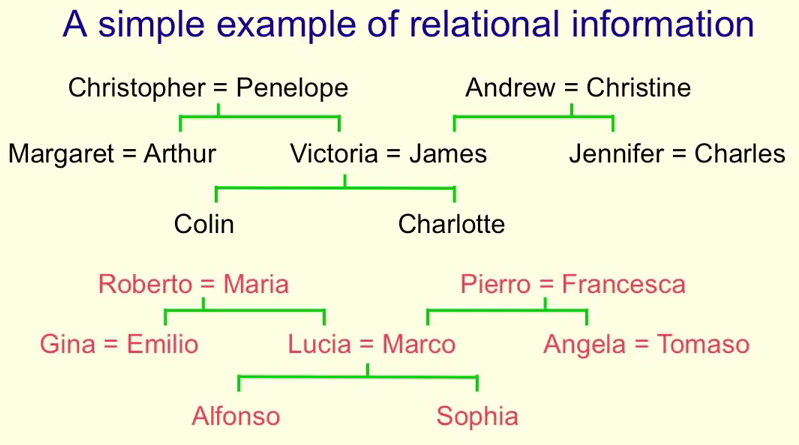
\includegraphics[scale=.5]{../Figuras/Hinton/ArbolGenealogico.png}
   \caption{Ejemplo de dos árboles genealogicos de familias nucleares.}
  \label{fig:arbolG}
  \end{figure}

En el árbol anterior se pueden apreciar que existen las siguientes 12 relaciones entre personas; hijo, hija, sobrino, sobrina, padre, madre, tío, tía, hermano, hermana, esposo, esposa. Y vamos a tener la siguientes proposiciones para denotarlas se la siguiente forma; 

\begin{itemize}
 \item (Colin tiene-padre James)
 \item(Colin tiene-madre Victoria)
 \item(James tiene-esposa Victoria)
\end{itemize}
La tarea objetivo: \textit{Que la red siguiente indique la segunda persona de la tercia, dados los valores en las dos primeras posiciones.} Si tenemos los valores [nombre entrada] [tiene-relación] [nombre salida], con los dos primeros datos nos debe dar el tercer dato.
Por ejemplo si nos preguntamos si Victoria tiene esposo, debería  darme como respuesta James. Puede ser que la respuesta no sea única, por ejemplo si pregunto si Charlotte tiene tío  hay dos respuestas posibles Arthur y Charles. No esperamos que la red haga nada lógico cuando no existe la relación. Solamente la probaremos con las relaciones que estén definidas en el árbol y por consiguiente en nuestro conjunto de entrenamiento. 

Entonces lo primero que tenemos que hacer es ver cómo codificar a las personas y a las relaciones, 
retomando el concepto de one hot encoding, es lo que vamos a hacer. Al ver la \fref{RedHinton86} vamos a tomar en la parte de abajo de la red neuronal que representa a las entradas, las codificaciones para la persona y el tipo de relación, lo que vamos a tener a la salida van a ser neuronas que representan a la segunda persona es la que está relacionada con la primera y es la que podemos la que podemos preguntar.

Lo que decidieron hacer en esta red, es no introducir sesgos inicio, pero hacer que la red por medio de su entrenamiento descubra una codificación compacta, donde se codifique juntos o con algún elemento en común, aquellos elementos que si tienen cosas en común, a esto se le llama hacer un auto codificador un encoder. 

El diseño de la red por capa se propones de la siguiente forma:

\begin{itemize}
 \item Capa uno:
 \begin{itemize}
  \item 24 neuronas de entrada (una para cada persona).
  \item 12 neuronas de entrada (una para cada relación).
 \end{itemize}
\item Capa dos:
 \begin{itemize}
  \item 6 neuronas conectadas con las 24 personas.
  \item 6 neuronas conectadas con las 12 relaciones.
 \end{itemize}
\item Capa tres:
 \begin{itemize}
  \item 12 neuronas conectadas a todas las neuronas en la capa 2.
 \end{itemize}
\item Capa cuatro:
 \begin{itemize}
  \item 6 neuronas conectadas a todas las neuronas en la capa 3.
 \end{itemize}
\item Capa cinco:
 \begin{itemize}
  \item 24 neuronas de salida, una para cada persona relacionada con la de entrada.
 \end{itemize}

\end{itemize}

Las datos de entrada son: 112 proposiciones, 100 utilizadas para entrenamiento, con 1500 iteraciones.

 La estructura de esta red la \fref{fig:RH86} en observen que no es una capa completamente conectada con la siguiente sino que ambos tipos de datos dan origen a dos regiones distintas, primero tenemos a la persona script en one-hot encoding por otro lado tenemos a la red, sin embargo vamos a tratar de y representar mejor esos datos y tratar de capturar si tienen algo en común entre ellas y eso lo vamos a lograr haciendo que la red misma descubra una forma compacta de representar a esas personas. 

 
  \begin{figure}[h]
   \centering
   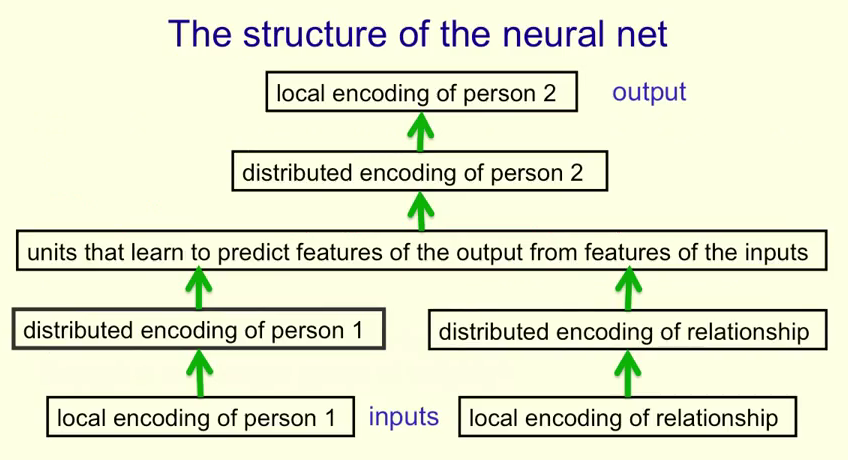
\includegraphics[scale=.5]{../Figuras/Hinton/RedHinton86.png}
   \caption{Estructura propuesta para la red neuronal de parentesco familiar.}
  \label{fig:RH86}
  \end{figure}

   Empezamos con 24 neuronas de entrada, después vamos a poner una mini capa, que solamente afecta, a estas neuronas y va a tener 6 neuronas eso quiere decir que la red neuronal tendrá que descubrir alguna manera de representar a las 24 personas con solamente 6 bits. Esta codificación le ayuda a predecir correctamente la persona que estamos buscando. Lo mismo vamos a hacer con el tipo de relaciones, había 12 en las neuronas de entrada, le vamos a reducir a 6 neuronas. Una vez que la red ha pasado por este cuello de botella, ha codificado así nuestros datos simbólicos, vamos a tener es una capa donde, ahora si conectamos todos contra todos es como si estas dos capas de pronto se fueran a pegar y se volvieran una. Estos van a estar conectados con todos estos esto es realmente lo que correspondería a nuestra capa de siempre nuestra capa oculta. Después vamos a tener que hacer el proceso inverso, en principio esta red de capa nos va a permitir encontrar  qué relación tienen dos personas, pero si queremos poder predecir la otra relación entonces necesitamos partir de lo que encontremos.
 
 Se va a reconstruir las características de la segunda persona, (se va a hacer el proceso inverso) vamos a tener también un codificador pero  trataremos de predecir a la persona correcta con solamente seis neuronas, es decir, la segunda persona de la relación va a estar codificada en términos de los vínculos que tenga con las otras personas que existen en el conjunto. Una vez que ya logramos obtener esa codificación, tenemos que decodificarla y representarla nuevamente con 24 neuronas en la capa de salida, una por cada persona. Si logramos lo anterior nuestro código compacto de la penultima capa se puede descomprimir sin pérdida en la respuesta.

Las seis neuronas ocultas en el cuello de botella conectado a la entrada representa las características de las personas que son útiles para predecir la salida, tales como, la rama del árbol genealógico al que pertenece.
La capa central aprende cómo las características predicen otras características. Por ejemplo, la persona de entrada es de generación 3 y la relación requiere que la respuesta sea una generación más, entonces implica que la persona de salida es de la generación 2.

  
\subsection{Codificacion de los datos de entrada}

Lo primero que tenemos que hacer es, conseguir todos los datos ´para alimentar a nuestra red y codificarlos como acabamos de ver. Para eso tenemos un archivo escrito a mano (ver \fref{fig:ejData}) donde se hicieron tuplas con todas las relaciones posibles y se describe quién está relacionado con quién, al menos en una de las direcciones. En las relaciones que son simétricas se reutiliza la información para que sea menos tedioso de leer, entonces si ya tenemos las relaciones de X tiene padre Y, tambien tenemos las relaciones de Y tiene hijo X.

  \begin{figure}[h]
   \centering
   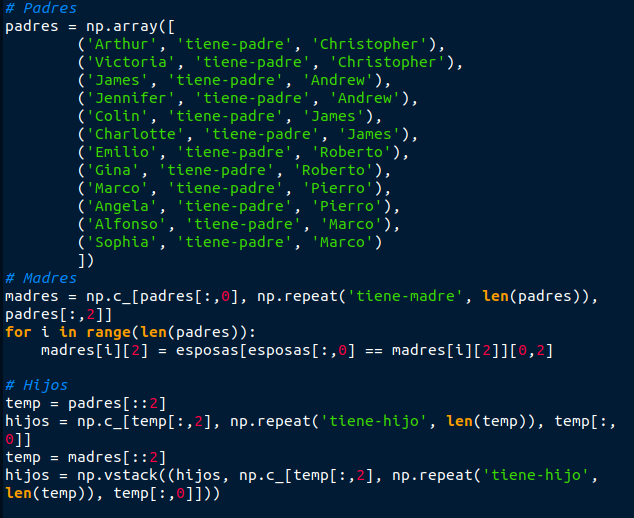
\includegraphics[scale=.5]{../Figuras/Hinton/data.png}
   \caption{Fragmento del archivo, con los datos utilizados para el ejercicio.}
  \label{fig:ejData}
  \end{figure}


Una vez que tenemos todas estas duplas las podemos cargar dentro de nuestro archivo donde hagamos la red. Es en ese archivo donde verificaremos que tenemos las 111 combinaciones, pero solamente 104 son entradas distintas, (recordemos el caso confuso, de los dos tíos). 

Ya te que nos aseguramos que este todo bien relacionado podemos hacer las entradas que recibira la red, que son solo los dos primero datoss de la tupla, ([nombre],[tiene-relacion]). 

A continuación tenemos que revisar las salidas, que serían todas las personas posibles, y todas las relaciones. Esto con one-hot encoding, se codifica a las personas posibles en un solo vector y a cada una se le asigna un lugar en este, así si James fue nuestra tercera persona en codificarse este ocupara el tercer lugar, y el vector se verá así $[0,0,1,0,\dots,0]$. Hacemos lo mismo para las relaciones, son solo 12 relaciones así que si tenemos la relación tiene-Tio, después de tiene-Padre y este fue el primero en codificarse, el vector para tiene-Tio se verá  así $[0,1,0,0,0,0,0,0,0,0,0,0]$. 

La primera persona va a corresponder con la primera neurona, la segunda persona con la segunda neurona, la tercera con la siguiente neurona y así sucesivamente. 

Vamos a dividir las muestras en dos conjuntos, el conjunto de entrenamiento para juntar los pesos y un conjunto de prueba para averiguar si es capaz de hacer predicción. Para crear estos conjuntos vamos a utilizar  una función que revuelva aleatoriamente, todas las relaciones posibles, utilizaremos 100 relaciones al entrenamiento y 4 para el de prueba. Como la arquitectura de la red ya está fija y lo único que vamos a hacer es tratar de ajustar los pesos.

Un tip, siempre la primera vez que se programe una red, se fija la semilla (para los muestreos aleatorios), lo que esto logrará hacer es que siempre que corre en el programa va a salir exactamente el mismo resultado. Al programar redes neuronales en varios pasos, como vamos a utilizar muestreos aleatorios, se piden números al azar. Si prueban en valores y funciona muy bien la próxima vez que ejecuten ese código no van a volver a obtener el mismo resultado y eso puede llegar a ser frustrante o puede complicar  el proceso de depuración e incluso el proceso de recuperar una red que estaba funcionando bien. 

No hay segos para esta red, porque  en el ejercicio no tendríamos porque predisponernos a suponer algo y fue así como lo plantearon, funcionó bien. 

\subsection{Alimentación hacia adelante}

Vamos a ver ahora cómo se lleva a cabo la alimentación hacia adelante, recordemos que tenemos que calcular dos cosas, la combinación lineal de los valores de activación de la capa anterior \ref{eq:uno} y sobre ella aplicarle la función de activación \ref{eq:dos}.

\begin{equation}
 a_{j}^{(l+1)} = g\left(\sum_{j}\Theta_{i,j}^{(l)}a_{j}^{(l)} \right)
 \label{eq:uno}
\end{equation}

\begin{equation}
 g = \dfrac{1}{1+e^{-x}}
 \label{eq:dos}
\end{equation}

Esto se puede hacer en manera matricial multiplicando en la matriz de pesos por los valores de activación, donde $a_{j}^{(l)}$  es el valor de activación de la neurona  $i$  en la capa  $l$ y $\Theta_{i,j}^{(l)}$ es el peso del arista que conecta a la neurona  $a_{j}^{(l)}$ con la neurona $a_{j}^{(l+1)}$.

$$
 \begin{bmatrix}
  a_{0}^{(l+1)}\\
  a_{1}^{(l+1)}\\
  \dots\\
  a_{n}^{(l+1)}\\
 \end{bmatrix}
 = g \left( 
  \begin{bmatrix}
  \theta_{10}^{(l)} & \dots & \theta_{1n}^{(l)}\\
  \dots \\
  \dots\\
  \theta_{n0}^{(l)} & \dots & \theta_{nn}^{(l)}\\
 \end{bmatrix}
 \begin{bmatrix}
  a_{0}^{(l+1)}\\
  a_{1}^{(l+1)}\\
  \dots\\
  a_{n}^{(l+1)}\\
 \end{bmatrix}
 \right)
 $$

  \begin{figure}[H]
   \centering
   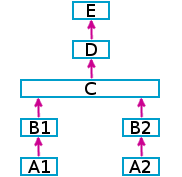
\includegraphics[scale=.5]{../Figuras/Hinton/RedRelaciones.png}
   \caption{Arquitectura de la red.}
  \label{fig:redArq}
  \end{figure}

El número de conexiones que se sugieren son las siguientes, teniendo en cuenta la arquitectura de la red que la podemos ver en la \fref{fig:redArq}:

\begin{itemize}
 \item $WA1\rightarrow(6*24)=144$ 
 \item  $WA2\rightarrow(6*12)=72$
 \item $WB1\rightarrow(12*6)=72$
 \item $WB2\rightarrow(12*6)=72$
 \item $WC\rightarrow(6*12)=72$
 \item $WD\rightarrow(24*6)=144$
\end{itemize}

En la primera capa tenemos dos bloques de neuronas, el $A1$ para meter los datos de las 24 personas y el $A2$ para meter las 12 relaciones posibles, estos van a tener de salida 6 neuronas cada bloque para los encoders. Las capas $B1$ y $B2$ son las encargadas de comprir la infomación, los encoders y estos hacen una conexión completa con la capa $C$, con 72 pesos por cada capa. La capa $C$ es la encargada de ver las características, como la información que tiene esta comprimida en 6 bits, ahora va a tener una salida de 12 bits para poder decodificar los datos, es decir tiene $6x12=144$ pesos. 
La capa $D$ es la encargada de decodificar los 6 bits que salen del bloque $C$ en 24 bits que es lo que necesitamos, uno para cada persona, entonces el bloque $D$ tiene $24x6=144$ pesos.

Así tenemos un total de 576 pesos, cuyo valor debe ser ajustado.

Entonces en el algoritmo de propagación hacia delante, lo que tenemos es el producto de los pesos por los valores de activación y después la función logística, para calcular los valores de activación de la siguiente capa. vemos que primero se realice esta operación nada más para el auto encoder del lado izquierdo. Después hacemos lo mismo pero para las entradas y pesos que conectan la capa $A2$ con $B2$. 

Una vez que obtuvimos ambos resultados unimos ambos elementos para que así se conecten todos contra todos en la capa $C$ y hacemos de nuevo el producto de los pesos por los valores de activación y después la función logística, se procede igual con $D$ y $E$ con sus respectivos valores.

Vamos a guardar todas las variables de salida para usarla en la retropropagación. De este modo tendremos acceso a los valores de activación en las combinaciones lineales después de haber ejecutado. 

Para la red, vamos a tener los métodos indispensables, un constructor donde podríamos asignar de pesos que ya hubiéramos sacado de algún otro lado.
Necesitamos un método que nos permita colocar todos los matrices de pesos en un solo vector entonces lo que hace es aprender todas estas matrices de pesos y ponerles una encima de la otra esta es una forma de tener los parámetros del algoritmo de entrenamiento como un vector. 

Después necesitamos una función auxiliar que lo que se encarga es de reconstruir todas estas matrices a partir de un vector, estos son métodos interesantes para poder probar qué es lo que estamos haciendo, por ejemplo hacer algo que jamás se debe de hacer podemos inicializar nuestra  red poniendo solamente unos en las matrices de pesos. Esto jamás se debe de hacer cuando intenten entrenar una red porque no va a aprender absolutamente nada, si todos los pesos son iguales, todas las componentes del cliente son iguales y todo el tiempo va a empeorar o va a mejorar para algunos ejemplares pero se va a descomponer para otros. entonces este método nos sirve para ver que cuando programamos el fit forward hayamos hecho algo que tenga sentido.

  \begin{figure}[H]
   \centering
   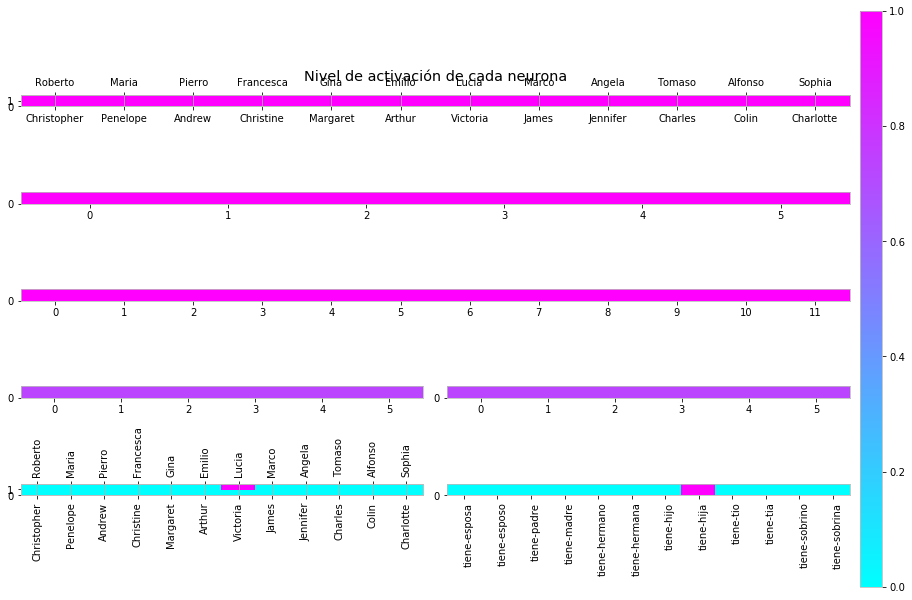
\includegraphics[scale=.5]{../Figuras/Hinton/r1.png}
   \caption{Red incializda con todos pesos en un mismo valor. Si todos los pesos de la red son ideinticos no tendremos una actualización de pesos atravez de las capas, provocando que nunca llegue a dar respuestas. Esta red nunca aprendería.}
  \label{fig:r1}
  \end{figure}


Entonces la siguiente fase es cuando nos mandan un conjunto de datos y queremos evaluarlos a través de la red de la función de la red y obtener los valores de salida. Cómo de estos datos de entrenamiento que separan el conjunto en personas y relaciones, se manda a llamar el método feedforward, con los datos del conjunto de prueba y finalmente  una vez que fueron programadas estas funciones vamos probar si realmente está funcionando el primer paso pues es crear una instancia del objeto, asignarle los unos que podemos para decir básicamente como puede verse y tratar de aplicar el feef forward. 

 Necesitamos visualizar qué es lo que pasó y esto es lo que hacemos con una función auxiliar que permite graficar lo que está sucediendo, ese está en el archivo plot.py del zip de Hinton del curso. Así que vamos a poder ver lo que estamos haciendo en la parte de abajo de esta gráfica \fref{fig:graf} podemos ver a las personas podemos ver las relaciones y los colores azules indican ceros. Entonces en un principio cuando pusimos los pesos con el mismo valor, dadas las entradas que tenía decir que tenía alta probabilidad de tener relación con todos o ninguno, y cuando la red ya está entrenada nos debe indicar solo una celda en color azul que es a la que pertenece.
 
  \begin{figure}[H]
   \centering
   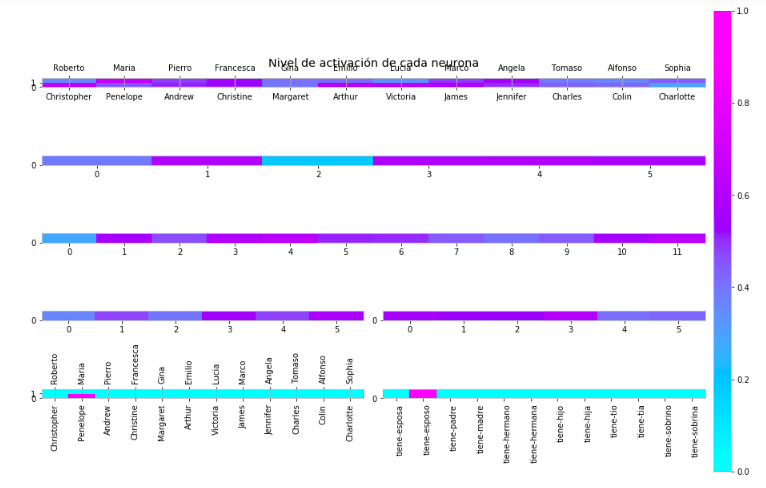
\includegraphics[scale=.5]{../Figuras/Hinton/graficaColores.png}
   \caption{Red con feedforward diferentes pesos, pero sin entrenar.}
  \label{fig:graf}
  \end{figure}

\subsection{Entrenamiento}

\subsection{Momentum y decaimiento de los pesos}

\subsection{Ejecución del entrenamiento}

    \begin{figure}[h]
   \centering
   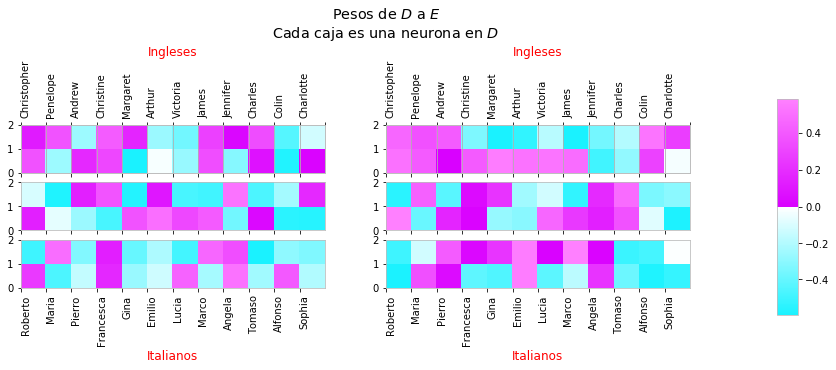
\includegraphics[scale=.5]{../Figuras/Hinton/r2.png}
   \caption{Resoluciones.}
  \label{fig:r2}
  \end{figure}

    \begin{figure}[h]
   \centering
   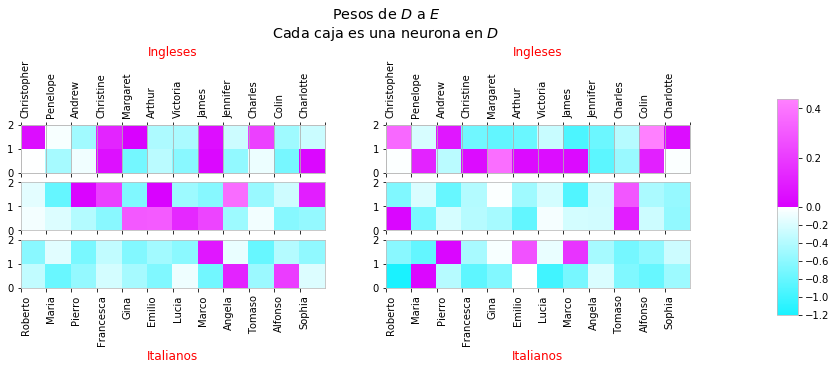
\includegraphics[scale=.5]{../Figuras/Hinton/r3.png}
   \caption{Resoluciones.}
  \label{fig:r3}
  \end{figure}


 
